\documentclass[a4paper,twoside]{article}
\usepackage[T1]{fontenc}
\usepackage[bahasa]{babel}
\usepackage{graphicx}
\usepackage{graphics}
\usepackage{float}
\usepackage[cm]{fullpage}
\pagestyle{myheadings}
\usepackage{etoolbox}
\usepackage{setspace} 
\usepackage{lipsum} 
\setlength{\headsep}{30pt}
\usepackage[inner=2cm,outer=2.5cm,top=2.5cm,bottom=2cm]{geometry} %margin
\usepackage{tabularx}
\usepackage[backend=biber, style=verbose-note]{biblatex}
\addbibresource{referensi.bib}
\usepackage{subcaption}
% \pagestyle{empty}

\makeatletter
\renewcommand{\@maketitle} {\begin{center} {\LARGE \textbf{ \textsc{\@title}} \par} \bigskip {\large \textbf{\textsc{\@author}} }\end{center} }
\renewcommand{\thispagestyle}[1]{}
\markright{\textbf{\textsc{AIF184001/AIF184002 \textemdash Rencana Kerja Tugas Akhir \textemdash Sem. Ganjil 2026/2027}}}

\newcommand{\HRule}{\rule{\linewidth}{0.4mm}}
\renewcommand{\baselinestretch}{1}
\setlength{\parindent}{0 pt}
\setlength{\parskip}{6 pt}

\onehalfspacing

\begin{document}
	
	\title{\@judultopik}
	\author{\nama \textendash \@npm} 
	
	%tulis nama dan NPM anda di sini:
	\newcommand{\nama}{Owen Lianggara}
	\newcommand{\@npm}{6182301025}
	\newcommand{\@judultopik}{Fuzzy Inference System (FIS) untuk Prediksi Kepribadian Seseorang Berdasarkan Tulisan Tangan} % Judul/topik anda
	\newcommand{\jumpemb}{1} % Jumlah pembimbing, 1 atau 2
	\newcommand{\tanggal}{06/03/2026}
	
	% Dokumen hasil template ini harus dicetak bolak-balik !!!!
	
	\maketitle
	
	\pagenumbering{arabic}
	
	\section{Deskripsi}
	Sejak lama, analisis dan penilaian kepribadian sudah menjadi kebutuhan di berbagai bidang, yaitu pendidikan, 
	rekrutmen sumber daya manusia, konseling, dan sebagainya. Kebutuhan ini terus meningkat untuk menilai bagaimana 
	seseorang mengenal dirinya sendiri dan membantu memahami karakter dan kepribadian seseorang dalam bersosialisasi, 
	yang memunculkan salah satu pendekatan untuk mempelajari hubungan antara kepribadian seseorang dengan tulisan tangannya, 
	yaitu grafologi. Grafologi merupakan metode ilmiah untuk mengenali, menilai, dan memahami kepribadian penulis melalui 
	bentuk dan pola kata dalam tulisan tangan \footcite{rahiman2013habit}.

	% (bahas secara psikolog dan dari sisi cara berpikir, jangan langsung teknis)
	Grafologi \footcite{hemlata2018personality} menganalisis kepribadian seseorang melalui bentuk fisik dari hasil menulis. Setiap orang memiliki tulisan yang berbeda-beda dan dalam proses kegiatan menulis, aktivitas tersebut bukan dilakukan
	oleh tangan, melainkan otak. Sehingga, setiap bentuk goresan tulisan yang dibuat menggambarkan bagaimana otak berperilaku. Dalam grafologi, tulisan tangan adalah aktivitas temporal, spasial, dan simbolik yang merefleksikan tempramen 
	bawaan dan bawah sadar penulis\footcite{Marano2021Graphology}. Ada 200 tanda grafologis yang dimasukkan ke dalam tujuh kategori, beberapa darinya dapat dilihat pada Tabel 1. Fitur-fitur tulisan tangan dapat lebih dari fitur yang telah 
	disebutkan dari sumber lain atau dapat digabungkan antarfitur sehingga menciptakan fitur baru setelah dilakukan analisis mendalam.
	\begin{table}[H]
		\caption{Fitur Analisis Tulisan Tangan. Sumber: Hemlata et al. (2018).}
		\label{tab:tabel_fitur}
		\begin{tabularx}{\textwidth}{|l|X|}
			\hline
			\textbf{Fitur} & \textbf{Penjelasan} \\
			\hline
			Zona & Analisis tiap zona (upper, middle, dan lower) dari huruf-huruf tertentu. Ilustrasi mengenai Zona dapat dilihat pada Gambar 1.a, 
			di mana beberapa huruf, seperti huruf b memiliki zona atas sedangkan huruf p memiliki zona bawah. \\
			\hline
			Kemiringan baseline & Ilustrasi kemiringan baseline dapat dilihat pada Gambar 1.b. Kemiringan pada satu baris tulisan dibagi menjadi tiga, yaitu miring ke atas, lurus horizontal, 
			dan miring ke bawah. \\
			\hline
			Kemiringan huruf & Ilustrasi kemiringan huruf dapat dilihat pada Gambar 1.c. Kemiringan pada tiap huruf dibagi menjadi tiga, yaitu miring ke kiri, tegak, dan miring ke kanan. \\
			\hline
			Ukuran margin & Sebuah kalimat atau paragraf yang sudah ditulis pada kertas kosong akan memiliki ukuran jarak antara 
			tulisan dengan batas kertas. \\
			\hline
			Ukuran tulisan & Ukuran tulisan didapat dengan mengukur tinggi tulisan dengan tiga kategori, yaitu besar, sedang, dan kecil, seperti pada ilustrasi Gambar 1.d. \\
			\hline
			Tekanan saat menulis & Tekanan saat menulis ditunjukkan melalui ketebalan dari hasil tulisan pada ilustrasi Gambar 1.e. Ketebalan tersebut memiliki 
			tiga kategori, yaitu berat, sedang, dan ringan. \\
			\hline
			Jarak antar kata & Jarak antara kata pertama dengan kata kedua secara konsisten, seperti pada ilustrasi Gambar 1.f. Jarak antar kata dibagi menjadi dua 
			kategori, yaitu lebar dan sempit. \\
			\hline
		\end{tabularx}
	\end{table}

	\begin{figure}[H]
		\centering
		\begin{subfigure}{0.45\textwidth}
			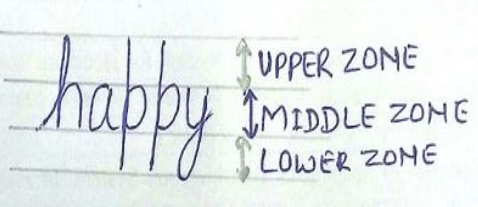
\includegraphics[width=\linewidth]{images/Zona.png}
			\caption{Zona}
		\end{subfigure}
		\hfill
		\begin{subfigure}{0.45\textwidth}
			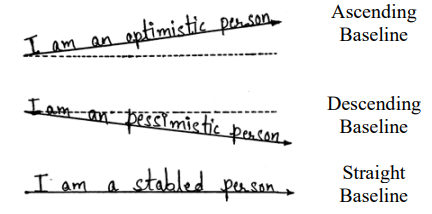
\includegraphics[width=\linewidth]{images/Baseline.png}
			\caption{Kemiringan baseline}
		\end{subfigure}
		\begin{subfigure}{0.45\textwidth}
			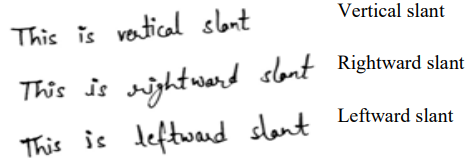
\includegraphics[width=\linewidth]{images/Huruf miring.png}
			\caption{Kemiringan huruf}
		\end{subfigure}
		\hfill
		\begin{subfigure}{0.45\textwidth}
			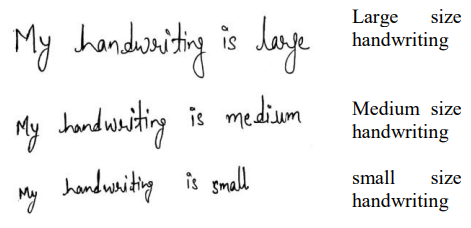
\includegraphics[width=\linewidth]{images/Ukuran.png}
			\caption{Ukuran tulisan}
		\end{subfigure}
		\begin{subfigure}{0.45\textwidth}
			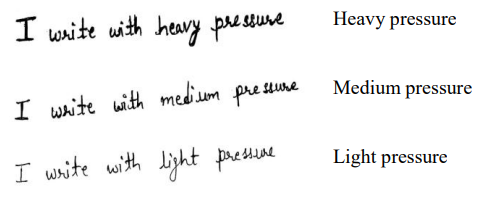
\includegraphics[width=\linewidth]{images/Tekanan.png}
			\caption{Tekanan}
		\end{subfigure}
		\hfill
		\begin{subfigure}{0.45\textwidth}
			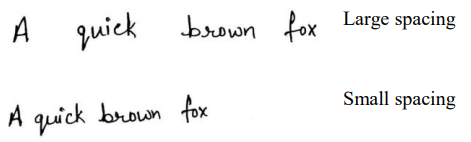
\includegraphics[width=\linewidth]{images/Jarak antar kata.png}
			\caption{Jarak antar kata}
		\end{subfigure}
		\caption{Ilustrasi contoh fitur-fitur tulisan tangan. Sumber: Hemlata et al. (2018).}
		\label{fig:fitur-tulisan}
	\end{figure}

	Melalui fitur-fitur tulisan tangan tersebut, gralofolog dapat menilai kepribadian seseorang. Namun, cara tersebut tergolong sebagai cara yang tradisional karena pada praktiknya, pendekatan 
	yang dilakukan oleh grafolog memiliki beberapa kekurangan, di mana hasil penilaian tidak luput dari subjektifitas grafolog sehingga dapat menyebabkan  ketidakkonsistenan penilaian antar grafolog. 
	Ketidakkonsistenan tersebut akan menyulitkan proses analisa terhadap kepribadian seseorang yang sedang diteliti dan mungkin dapat terjadi dalam waktu yang lama, sampai grafolog lainnya menyatakan 
	hasil yang berbeda. Selain itu, dalam kasus tertentu, grafolog dapat kesulitan dalam menilai fitur tulisan secara pasti, seperti pada kasus di mana sebuah tulisan dinilai "agak tebal", tapi dalam 
	penilaian lainnya dinilai "tidak tebal". Perbedaan penilaian tersebut dapat terjadi karena perbedaan subjektifitas antar grafolog sehingga dengan deskripsi linguistik, seperti “agak”, “sedikit”, 
	“kuat”, dan deskripsi lainnya bersifat kabur, tidak terlihat batas jelasnya secara presisi. Oleh karena itu, perlunya pendekatan komputasional agar dapat melakukan analisis dan penilaian dari bentuk fisik tulisan secara jelas dan konsisten.
	
	Salah satu metode komputasi dalam memprediksi kepribadian seseorang adalah menggunakan deep learning \footcite{gagiu2025detection}. Dengan menggunakan Convolutional Neural Network (CNN) 
	untuk mengolah data tulisan, model berfokus untuk mencari pola tersembunyi pada tulisan melalui perubahan bobot tiap epoch pelatihan dengan hasil akhir berupa 
	\textit{score Myers-Briggs Type Indicator} (MBTI). Metode lain yang dapat digunakan untuk memprediksi kepribadian seseorang adalah menggunakan Fuzzy Inference System (FIS) yang dirancang khusus untuk menangani kasus samar pada bentuk tulisan. 
	FIS mengubah penilaian pada istilah linguistik menjadi nilai numerik melalui fungsi keanggotaan dan aturan IF-THEN. Salah satu implementasi dari FIS 
	untuk permasalahan ini telah diaplikasikan dengan menggunakan FIS menggunakan metode Mamdani \footcite{ghods2023personality}. Dengan menggunakan sembilan 
	\textit{fuzzy system} yang terdiri dari dua \textit{fuzzy set}, yaitu \textit{LOW} dan \textit{HIGH}, model mampu memprediksi dengan tingkat akurasi 
	sebesar 82.5\%.

	Tugas akhir ini menggunakan model karakteristik \textit{Big five personality}. \textit{Big five personality} atau yang dikenal dengan model OCEAN merupakan singkatan dari lima kepribadian, yaitu \textit{Openness}, \textit{Conscientiousness}, \textit{Extraversion},
	\textit{Agreeableness}, dan \textit{Neuroticism}, dengan penjelasan setiap kepribadian dapat dilihat pada Tabel 2 \footcite{JohnNaumannSoto2008BigFive}. Model kepribadian ini bermula dari Allport and Odbert's (1936) mengidentifikasi kurang lebih 18.000 istilah 
	kepribadian pada kamus bahasa inggris. Penemuan Allport and Odbert's menjadi awal mula dari penelitian selanjutnya. Sehingga karena jumlahnya yang sangat besar, dibutuhkan metode untuk mereduksi tiap kepribadian tersebut. Pada penemuan selanjutnya, Catell (1943) 
	mengambil 4.500 istilah kepribadian dari 18.000 istilah dan mereduksinya menjadi 35 variabel. Dengan memanfaatkan 35 variabel tersebut, Catell meringkasnya menjadi 12 faktor setelah menemukan korelasi antar kepribadian yang saling berkaitan dan dapat dijadikan 
	sebagai satu kepribadian, sehingga mendasari penemuan kuisoner 16 \textit{Personality Factors}. Penemuan selanjutnya, Fiske (1949) yang menemukan lima struktur faktor karakteristik, kemudian diperkuat oleh penemuan Tupes dan Christal (1961) dengan hasil yang serupa 
	dari \textit{Cattel's Variable List}, yang sekarang diketahui sebagai \textit{the Big Five}.
	\begin{table}[H]
		\caption{Model OCEAN. Sumber: John, Naumann dan Soto.}
		\label{tab:tabel_ocean}
		\begin{tabularx}{\textwidth}{|l|X|}
			\hline
			\textbf{Karakteristik} & \textbf{Penjelasan} \\
			\hline
			Openness & Menggambarkan keluasan, kedalaman, orisinalitas, dan kompleksitas kehidupan mental serta pengalaman seseorang. \\
			\hline
			Conscientiousness & Kontrol impuls yang ditetapkan secara sosial yang berorientasi pada tugas dan tujuan, seperti berpikir sebelum bertindak, menunda kepuasan, mengikuti norma dan aturan, serta merencanakan, mengatur, 
			dan memprioritaskan tugas. Sehingga kepribadian ini cenderung berhati-hati mengikuti aturan sosial yang disepakati. \\
			\hline
			Extraversion & Keterbukaan terhadap sosial dan material dunia, termasuk bersosialisasi, aktivitas, ketegasan, dan positif secara emosional. \\
			\hline
			Agreeableness & Perbandingan antara orientasi prososial dan komunal terhadap orang lain dengan antagonisme, dan mencakup sifat-sifat seperti altruisme, kelembutan hati, kepercayaan, dan kerendahan hati. \\
			\hline
			Neuroticism & Stabilitas emosional, sikap tenang, dan stabil, tapi dengan emosional negatif, seperti merasa cemas, gugup, sedih, dan tegang. \\
			\hline
		\end{tabularx}
	\end{table}

	Pada tugas akhir ini, perangkat lunak prediksi karakteristik seseorang berdasarkan tulisan tangan diimplementasikan secara menyeluruh, mencakup antarmuka, metode \textit{fuzzy inference system}
	yang telah dipilih, serta dashboard hasil yang transparan dari penilaian setiap fitur dan hasil akhir. Dalam perangkat lunak, sistem harus dapat menerima input berupa pindai atau foto
	tulisan tangan yang selanjutnya dilakukan \textit{image preprocessing} agar setiap fitur dapat dibaca tanpa gangguan eksternal dari gambar. Setelah sistem menilai berdasarkan 
	hasil pindai atau foto, dashboard akan menunjukkan hasil kepada pengguna sehingga pengguna dapat melihat penilaian berupa penilaian numerik setiap fitur dan hasil akhir berupa tipe kepribadian
	dari \textit{Big five personality}.

	\section{Rumusan Masalah}
	% Tuliskan rumusan dari masalah yang akan anda bahas pada tugas akhir ini. Rumusan masalah biasanya berupa kalimat pertanyaan. Gunakan penomoran untuk menuliskan rumusan masalah ini.
	Berikut ini adalah rumusan masalah yang diselesaikan dalam tugas akhir ini:
	\begin{enumerate}
		\item Bagaimana fitur-fitur tulisan tangan dapat dipilih untuk memprediksi karakteristik kepribadian?
		\item Bagaimana cara merancang dan mengimplementasikan sistem ekstraksi fitur tulisan tangan dari hasil pindai atau foto?
		\item Bagaimana membangun pemodelan, fungsi keanggotaan, dan aturan fuzzy pada Fuzzy Inference System yang mampu memprediksi kepribadian seseorang?
		\item Bagaimana cara merancang dan mengimplementasikan perangkat lunak FIS untuk prediksi kepribadian seseorang berdasarkan tulisan tangan?
		\item Bagaimana kinerja FIS yang dibangun dibandingkan dengan hasil tes kepribadian manual?
	\end{enumerate}

	\section{Tujuan}
	% Tuliskan tujuan dari topik tugas akhir yang anda ajukan. Tujuan penelitian biasanya berkaitan erat dengan pertanyaan yang diajukan di bagian rumusan masalah. Gunakan penomoran untuk menuliskan rumusan masalah ini, di mana tiap nomor berkaitan dengan nomor pada rumusan masalah.
	Berikut ini adalah tujuan yang ingin dicapai dalam tugas akhir ini:
	\begin{enumerate}
		\item Melakukan studi literatur dari berbagai sumber untuk menemukan fitur-fitur tulisan tangan yang relevan.
		\item Merancang dan mengimplementasikan sistem ekstraksi fitur tulisan tangan, seperti kemiringan huruf, jarak antar kata, dan sebagainya, dari pindai atau foto.
		\item Melakukan studi literatur, menganalisis, dan membangun model, fungsi keanggotaan, dan aturan FIS yang tepat dengan kasus prediksi kepribadian.
		\item Merancang dan membangun perangkat lunak untuk prediksi kepribadian seseorang berdasarkan tulisan tangan, termasuk pindai atau foto dan antarmuka hasil dari kalkulasi komputasi.
		\item Melakukan pengujian terhadap hasil dari perhitungan perangkat lunak dengan hasil tes kepribadian manual.
	\end{enumerate}

	\section{Deskripsi Perangkat Lunak}
	% Tuliskan deksripsi dari perangkat lunak yang akan anda hasilkan. Apa saja fitur yang disediakan oleh PL tersebut dan apa saja kemampuan dari PL tersebut. Perhatikan contoh di bawah ini:
	
	Perangkat lunak akhir yang akan dibuat memiliki fitur minimal sebagai berikut:
	\begin{itemize}
		\item Sistem dapat menerima input tulisan tangan berupa pindai atau foto.
		\item Sistem melakukan perhitungan dengan metode dari \textit{Fuzzy System Inference}
		\item Sistem menampilkan penilaian setiap karakteristik/fitur tulisan tangan pengguna.
		\item Sistem menampilkan kepribadian pengguna.
	\end{itemize}
	
	\section{Detail Pengerjaan Tugas Akhir}
	% Tuliskan bagian-bagian pengerjaan skripsi secara detail. Bagian pekerjaan tersebut mencakup awal hingga akhir skripsi, termasuk di dalamnya pengerjaan dokumentasi skripsi, pengujian, survei, dll.
	
	Bagian-bagian pekerjaan skripsi ini adalah sebagai berikut :
	\begin{enumerate}
		\item Studi literatur mengenai \textit{fuzzy logic}, teknik pembangunan \textit{rule} dan penerapan FIS terhadap masalah yang sama.
		\item Analisis kebutuhan perangkat lunak, yaitu fitur input, output kepribadian, dan sumber dataset.
		\item Melakukan perancangan sistem yang meliputi arsitektur, himpunan fuzzy, \textit{rule base}, dan desain antarmuka.
		\item Implementasi perangkat lunak dan sistem FIS.
		\item Melakukan pengujian, eksperimen, dan kinerja prediksi dari sistem FIS.
		\item Analisis metrik evaluasi dengan melakukan perbandingan terhadap kesesuaian pada hasil dataset.
		\item Menulis dokumen tugas akhir.
	\end{enumerate}
	
	\section{Rencana Kerja}
	Rincian capaian yang direncanakan di Tugas Akhir 1 adalah sebagai berikut:
	\begin{enumerate}
		\item Studi literatur mengenai grafologi dan penerapan FIS terhadap masalah yang sama.
		\item Analisis kebutuhan perangkat lunak, yaitu fitur input, output kepribadian, dan sumber dataset.
		\item Melakukan perancangan sistem yang meliputi arsitektur, himpunan fuzzy, \textit{rule base}, dan desain antarmuka.
		\item Menulis dokumen tugas akhir (TA 1).
	\end{enumerate}
	
	Sedangkan yang akan diselesaikan di Tugas Akhir 2 adalah sebagai berikut:
	\begin{enumerate}
		\item Implementasi perangkat lunak dan sistem FIS.
		\item Melakukan pengujian, eksperimen, dan kinerja prediksi dari sistem FIS.
		\item Analisis metrik evaluasi dengan melakukan perbandingan terhadap kesesuaian pada hasil dataset.
		\item Menulis dokumen tugas akhir (TA 2).
	\end{enumerate}
	
	\vspace{1cm}
	\centering Bandung, \tanggal\\
	\vspace{2cm} \nama \\ 
	\vspace{1cm}
	
	Menyetujui, \\
	\ifdefstring{\jumpemb}{2}{
		\vspace{1.5cm}
		\begin{centering} Menyetujui,\\ \end{centering} \vspace{0.75cm}
		\begin{minipage}[b]{0.45\linewidth}
			% \centering Bandung, \makebox[0.5cm]{\hrulefill}/\makebox[0.5cm]{\hrulefill}/2013 \\
			\vspace{2cm} Nama: \makebox[3cm]{\hrulefill}\\ Pembimbing Utama
		\end{minipage} \hspace{0.5cm}
		\begin{minipage}[b]{0.45\linewidth}
			% \centering Bandung, \makebox[0.5cm]{\hrulefill}/\makebox[0.5cm]{\hrulefill}/2013\\
			\vspace{2cm} Nama: \makebox[3cm]{\hrulefill}\\ Pembimbing Pendamping
		\end{minipage}
		\vspace{0.5cm}
	}{
		% \centering Bandung, \makebox[0.5cm]{\hrulefill}/\makebox[0.5cm]{\hrulefill}/2013\\
		\vspace{2cm} Nama: \makebox[3cm]{\hrulefill}\\ Pembimbing Tunggal
	}
\end{document}
